% !TEX TS-program = lualatex
\documentclass{vsureport}

\usepackage[dvipsnames]{xcolor}
\usepackage{listings}
\usepackage{enumitem}

\lstdefinelanguage{Kotlin}{
  comment=[l]{//},
  commentstyle={\color{gray}\ttfamily},
  emph={filter, first, firstOrNull, forEach, lazy, map, mapNotNull, println},
  emphstyle={\color{OrangeRed}},
  identifierstyle=\color{black},
  keywords={!in, !is, abstract, actual, annotation, as, as?, break, by, catch, class, companion, const,
    constructor, continue, crossinline, data, delegate, do, dynamic, else, enum, expect, external,
    false, field, file, final, finally, for, fun, get, if, import, in, infix, init, inline, inner,
    interface, internal, is, lateinit, noinline, null, object, open, operator, out, override,
    package, param, private, property, protected, public, receiver, reified, return, return@,
    sealed, set, setparam, super, suspend, tailrec, this, throw, true, try, typealias, typeof,
    val, var, vararg, when, where, while},
  keywordstyle={\color{NavyBlue}\bfseries},
  escapeinside={//(`}{`)},
  morecomment=[s]{/*}{*/},
  morestring=[b]",
  morestring=[s]{"""*}{*"""},
  ndkeywords={@Composable, @Preview, @Deprecated, @JvmField, @JvmName, @JvmOverloads, @JvmStatic,
    @JvmSynthetic, Array, Byte, Double, Float, Int, Integer, Iterable, Long, Runnable, Short,
    String, Any, Unit, Nothing},
  ndkeywordstyle={\color{BurntOrange}\bfseries},
  sensitive=true,
  stringstyle={\color{ForestGreen}\ttfamily},
  breaklines=true,              % включить перенос строк
  breakatwhitespace=false,      % разрешить перенос в любом месте, не только по пробелам
  postbreak=\mbox{\textcolor{red}{$\hookrightarrow$}\space}, % стрелка переноса (опционально)
  columns=flexible,             % гибкое выравнивание символов для корректного переноса
  basicstyle=\ttfamily\small,   % размер и шрифт текста
}

\begin{document} % начало документа 
% НАЧАЛО ТИТУЛЬНОГО ЛИСТА 
\begin{center} 
\hfill \break 
\large{МИНОБРНАУКИ РОССИИ}\\ 
\footnotesize{ФЕДЕРАЛЬНОЕ ГОСУДАРСТВЕННОЕ БЮДЖЕТНОЕ}\\  
\footnotesize{ОБРАЗОВАТЕЛЬНОЕ УЧРЕЖДЕНИЕ ВЫСШЕГО ОБРАЗОВАНИЯ}\\ 
\small{«ВОРОНЕЖСКИЙ ГОСУДАРСТВЕННЫЙ УНИВЕРСИТЕТ»}\\ 
\small{(ФГБОУ ВО «ВГУ»)}\\ 
\hfill \break 
\normalsize{Факультет прикладной математики, информатики и механики}\\ 
\hfill \break 
\normalsize{Кафедра математического обеспечения ЭВМ}\\ 
\hfill\break 
\large{Разработка мобильного приложения для отслеживания расписания на платформе Android}\\ 
\hfill \break 
\normalsize{Курсовая работа по дисциплине}\\ 
\normalsize{Б1.О.31 Проектирование информационных систем}\\ 
\hfill \break 
\normalsize{02.03.02 Фундаментальная информатика и информационные технологии}\\ 
\hfill \break 
\normalsize{Инженерия программного обеспечения}\\ 
\hfill \break 
\end{center} 

\normalsize{  
\begin{tabular}{l@{\hspace{4cm}}r}
Зав. кафедрой & \underline{\hspace{3cm}} \\
д.т.н., профессор Абрамов Г.В. & \underline{\hspace{3cm}} \\[1cm]
Обучающийся & \underline{\hspace{3cm}} \\
Вафин А.Р. & \underline{\hspace{3cm}} \\[1cm]
Руководитель & \underline{\hspace{3cm}} \\
к.ф.-м.н., доцент Болотова С.Ю. & \underline{\hspace{3cm}} \\
\end{tabular} 
}\\ 

\hfill \break 

\begin{center} Воронеж 2024 \end{center} 

\thispagestyle{empty} % выключаем отображение номера для этой страницы 
% КОНЕЦ ТИТУЛЬНОГО ЛИСТА 

\newpage
\thispagestyle{empty} % без номера страницы
\tableofcontents

\newpage
\section*{Введение}

В современном мире мобильные приложения стали неотъемлемой частью повседневной жизни, охватывая все новые аспекты человеческой деятельности. Особую значимость приобретает их использование в образовательной сфере, в частности для организации учебного процесса в высших учебных заведениях. Разработка специализированных приложений для отслеживания расписания занятий представляет собой актуальную задачу, обусловленную возрастающей цифровизацией образования и повсеместным использованием смартфонов студенческой аудиторией.

Актуальность разработки подобного приложения для платформы Android обусловлена несколькими ключевыми факторами. Во-первых, Android занимает лидирующие позиции на рынке мобильных операционных систем, что обеспечивает широкий охват пользовательской аудитории. Во-вторых, современные технологии разработки позволяют реализовать эффективную синхронизацию с университетскими базами данных через специализированные API. В-третьих, существует возможность внедрения дополнительных функций, таких как интеллектуальные уведомления, аналитика учебной нагрузки и персонализированные рекомендации, что способствует оптимизации образовательного процесса. \cite{ref1}

Таким образом, создание мобильного приложения для управления расписанием в вузе представляет собой научно-практическую задачу, решение которой может значительно повысить эффективность организации учебной деятельности. Перспективным направлением дальнейших исследований является интеграция технологий искусственного интеллекта для прогнозирования и адаптации учебного процесса под индивидуальные потребности студентов.


\newpage

\section*{1. Постановка цели и задач}
\addcontentsline{toc}{section}{1. Постановка цели и задач} % Добавляем в оглавление

Целью данной работы является разработка мобильного приложения для отслеживания расписания в вузе на платформе Android. Для достижения этой цели необходимо решить следующие задачи:

\begin{enumerate}
	\item Проектирование и реализация приложения, включая создание интерфейса, использование баз данных для хранения расписания и механизмов синхронизации для обновления данных в реальном времени.
	
	\item Реализация выбранного API, интеграция его в приложение и тестирование работы, включая написание кода для взаимодействия с API, обработку данных и обеспечение корректной работы всех функций приложения.
\end{enumerate}

\newpage

\section*{2. Анализ средств реализации}
\addcontentsline{toc}{section}{2. Анализ средств реализации} % Добавляем в оглавление

Для достижения поставленных целей и решения задач будут использованы следующие методы анализа и исследования:
\begin{enumerate}
\item Анализ существующих приложений для отслеживания расписания и API.
\item Проектирование пользовательского интерфейса с использованием методов UX/UI дизайна.
\item Разработка и тестирование программного кода приложения.
\end{enumerate}


\subsection*{2.1. Обзор существующих приложений}
\addcontentsline{toc}{subsection}{2.1. Обзор существующих приложений}
При анализе приложения "Расписание занятий" был выявлен ряд преимуществ. Одним из достоинств является возможность синхронизации данных с Google Sheets API, что обеспечивает актуальное отображение расписания. Еще одним преимуществом выступает функция добавления и редактирования заметок к каждому занятию, повышающая удобство использования. Простота интеграции с Google Sheets и быстрая загрузка данных также относятся к сильным сторонам данного решения. Однако приложение имеет существенные недостатки, среди которых отсутствие поддержки на новых версиях Android и невозможность отображения пар по числителю/знаменателю.\cite{ref2}
Приложение "Учебный календарь" демонстрирует другие преимущества. Важным достоинством является не только синхронизация с Google Sheets API, но и возможность персонализации интерфейса через изменение цветовой схемы. Особого внимания заслуживает реализация заметок о паре с функцией их включения и отключения, что предоставляет пользователям гибкость в настройке отображения информации. Еще одним значимым преимуществом стала поддержка отображения пар по числителю/знаменателю. Однако приложение страдает от перегруженного интерфейса и медленной загрузки данных, а также не предоставляет возможности самостоятельного выбора числителя/знаменателя.
На основании проведенного анализа было принято решение объединить сильные стороны обоих приложений, дополнив их новыми функциями. Ключевыми особенностями разрабатываемого решения станут: возможность изменения цветовой схемы интерфейса, реализация системы заметок о паре с функцией их отображения/скрытия, а также введение выбора роли (студент/преподаватель) и группы для студентов. Особое внимание уделено реализации самостоятельного выбора числителя/знаменателя, что обеспечит большую гибкость в работе с расписанием независимо от номера недели.

\subsection*{2.2. Обзор существующих языков программирования}
\addcontentsline{toc}{subsection}{2.2. Обзор существующих языков программирования} % Добавляем в оглавление

При сравнении Java и Kotlin выявлены существенные различия в подходах к разработке. Java, будучи зрелым языком, требует больше ручного управления кодом, включая написание геттеров, сеттеров и других шаблонных конструкций, что увеличивает объем работы и вероятность ошибок. В то же время Kotlin предлагает более высокоуровневый подход с автоматической генерацией boilerplate-кода, например, в data-классах, что делает разработку быстрее и удобнее.
В плане производительности оба языка компилируются в байт-код JVM, однако Kotlin предоставляет встроенные оптимизации, такие как null-безопасность и корутины, которые упрощают асинхронное программирование и снижают риск ошибок. Java, хотя и остается высокопроизводительным, требует ручной оптимизации, особенно при работе с памятью и многопоточностью.
Гибкость Kotlin проявляется в поддержке функционального программирования, включая лямбда-выражения и расширения функций, что позволяет писать более лаконичный и модульный код. Java, несмотря на добавление Stream API и лямбд, все еще уступает в этом отношении, требуя большего количества шаблонного кода.
Поддержка и сообщество Java остаются одними из самых больших, что делает язык надежным выбором для legacy-проектов. Однако Kotlin активно развивается, особенно в Android-разработке, и полностью совместим с Java, что позволяет использовать существующие библиотеки и постепенно переходить на более современный стек.
Тестирование в Kotlin упрощается благодаря лаконичному синтаксису и встроенным возможностям, таким как корутины, тогда как в Java для сложных сценариев часто требуются дополнительные библиотеки. 
В итоге Kotlin был выбран как более современный, безопасный и удобный язык, сочетающий производительность Java с улучшенным синтаксисом и инструментами.

\subsection*{2.3. Обзор существующих API}
\addcontentsline{toc}{subsection}{2.3. Обзор существующих API} % Добавляем в оглавление

Использование Google Sheets API для синхронизации данных имеет ряд существенных ограничений, что делает разработку собственного сервера более предпочтительным решением. Одним из основных недостатков является строгое ограничение на количество запросов в минуту, что может привести к задержкам или блокировке доступа при высокой нагрузке, тогда как собственный сервер позволяет гибко масштабировать ресурсы в зависимости от числа пользователей.
Еще одной проблемой Google Sheets API является сложность расширения функциональности, поскольку он не поддерживает такие возможности, как уведомления или аналитика, в то время как собственный сервер предоставляет полный контроль над логикой приложения и позволяет легко интегрировать дополнительные функции.
Изменение данных через Google Sheets также оказывается неудобным, так как требует ручного редактирования таблиц, что повышает риск ошибок, тогда как собственный сервер может быть оснащен удобной административной панелью для управления расписанием.
Производительность Google Sheets API оставляет желать лучшего при работе с большими объемами данных, вызывая задержки, в отличие от собственного сервера, который можно оптимизировать для быстрой обработки запросов.
Кроме того, Google Sheets API ограничен табличной структурой, что затрудняет работу со сложными данными, в то время как собственный сервер поддерживает различные форматы хранения, включая реляционные базы, обеспечивая большую гибкость.
Таким образом, собственный сервер предлагает значительные преимущества, включая полный контроль над данными, масштабируемость, удобство управления и расширяемость, что делает его оптимальным выбором для обеспечения стабильной и функциональной работы приложения.

\subsection*{2.4. Обзор существующих фреймворков для интерфейса}
\addcontentsline{toc}{subsection}{2.4. Обзор существующих фреймворков для интерфейса} % Добавляем в оглавление

При сравнении подходов к созданию пользовательского интерфейса явно прослеживаются ключевые различия между традиционной XML-версткой и современным Jetpack Compose. XML-верстка, несмотря на свою зрелость и обширную базу существующих решений, демонстрирует ряд существенных ограничений, таких как жесткое разделение логики и интерфейса, необходимость ручного управления View-элементами и сложности с динамическим обновлением контента. В противоположность этому, Jetpack Compose предлагает единый программный подход на Kotlin, где интерфейс описывается декларативно непосредственно в коде, что значительно упрощает разработку и поддержку.
С точки зрения производительности Compose обладает явными преимуществами благодаря своей системе "рекомпозиции", которая интеллектуально обновляет только измененные элементы интерфейса. В отличие от традиционной View-системы с ее глубокими иерархиями и ручной оптимизацией, Compose обеспечивает более эффективное использование ресурсов устройства, что особенно важно для современных требовательных приложений.
Гибкость Compose проявляется в простоте создания сложных анимированных интерфейсов и кастомизации компонентов. В то время как XML-верстка требует написания значительного объема кода для реализации нестандартных решений, Compose предоставляет встроенные инструменты для анимаций и позволяет легко создавать переиспользуемые компоненты.
Несмотря на то, что XML-верстка имеет более обширное сообщество и документацию из-за своей долгой истории, Jetpack Compose активно развивается при поддержке Google и постепенно становится новым стандартом в Android-разработке. Его возможность сосуществования с традиционными View позволяет осуществлять плавный переход на новые технологии.
В области тестирования Compose также предлагает более удобные решения со встроенными инструментами тестирования, что упрощает процесс проверки UI по сравнению с необходимостью использования дополнительных библиотек в случае XML-верстки.
Таким образом, Jetpack Compose был выбран как современный, производительный и гибкий фреймворк, который значительно ускоряет разработку интерфейсов за счет сокращения шаблонного кода и предоставления мощных инструментов для создания отзывчивых и интерактивных пользовательских интерфейсов.

\subsection*{2.5. Обзор существующих фреймворков базы данных}
\addcontentsline{toc}{subsection}{2.5. Обзор существующих фреймворков базы данных} % Добавляем в оглавление

При выборе подхода к работе с базами данных в Android-приложениях рассматривались два основных решения: нативный SQLite и библиотека Room. Нативный SQLite, являясь стандартным решением для Android, требует значительных усилий при реализации - разработчику необходимо вручную создавать таблицы, писать SQL-запросы и управлять соединениями, что приводит к большому объему шаблонного кода. В отличие от этого, Room предоставляет удобную абстракцию над SQLite, автоматически генерируя необходимый код на основе аннотаций, что значительно сокращает время разработки и уменьшает вероятность ошибок.
С точки зрения производительности оба подхода демонстрируют сопоставимые результаты, так как Room в конечном итоге использует тот же SQLite. Однако Room предлагает дополнительные оптимизации, такие как кэширование запросов и проверка их корректности на этапе компиляции, что позволяет избежать распространенных ошибок, характерных для ручного написания SQL-запросов. При этом нативный SQLite сохраняет преимущество при работе с особо сложными запросами, где может потребоваться тонкая ручная оптимизация.
Гибкость нативного SQLite проявляется в возможности выполнения произвольных запросов и полном контроле над структурой базы данных, однако это требует от разработчика глубоких знаний SQL и тщательного управления миграциями. Room, хотя и ограничивает некоторые низкоуровневые возможности, предоставляет удобные механизмы для работы с транзакциями и миграциями данных, существенно упрощая эти процессы. Особенно ценным является встроенная в Room поддержка LiveData и Flow, позволяющая легко реализовать реактивное обновление интерфейса при изменениях в базе данных.
Несмотря на то, что нативный SQLite имеет более обширную базу знаний и примеров благодаря своей долгой истории, Room активно развивается как часть Android Jetpack и становится стандартом для новых проектов. Его популярность постоянно растет, а сообщество разработчиков расширяется, что обеспечивает хорошую поддержку и наличие актуальных решений для типовых задач.
Важным преимуществом Room являются встроенные инструменты тестирования, такие как возможность создания временных баз данных в памяти, что существенно упрощает процесс написания и выполнения unit-тестов по сравнению с нативным SQLite, где требуется дополнительная настройка тестового окружения.
Таким образом, Room был выбран в качестве основного инструмента для работы с базами данных благодаря своей простоте использования, безопасности типов, отличной интеграции с другими компонентами Android Jetpack и возможности сосредоточиться на бизнес-логике приложения, а не на низкоуровневых деталях работы с SQLite.\cite{ref3}

\subsection*{2.6. Обзор существующих фреймворков для работы с сетью}
\addcontentsline{toc}{subsection}{2.6. Обзор существующих фреймворков для работы с сетью} % Добавляем в оглавление

При разработке сетевого слоя приложения рассматривались два основных подхода: низкоуровневый OkHttp и высокоуровневый Retrofit. OkHttp предоставляет полный контроль над HTTP-запросами, позволяя тонко настраивать все параметры соединения, однако требует значительного объема ручного кода для реализации типовых сценариев. В отличие от него, Retrofit предлагает декларативный подход через аннотированные интерфейсы, автоматизируя создание клиентов и обработку ответов, что существенно сокращает объем шаблонного кода.
С точки зрения производительности оба решения демонстрируют отличные результаты, поскольку Retrofit использует OkHttp в качестве транспортного уровня. OkHttp обеспечивает продвинутые оптимизации, включая поддержку HTTP/2, кэширование и сжатие данных, в то время как Retrofit добавляет удобную абстракцию поверх этих возможностей без потери эффективности.
Гибкость OkHttp проявляется в возможности создания кастомных интерцепторов и полного контроля над запросами, что критично для сложных интеграций. Retrofit, хотя и ограничивает некоторые низкоуровневые возможности, сохраняет доступ к базовым настройкам OkHttp и предоставляет удобные механизмы для адаптации ответов и обработки ошибок.
Оба решения имеют отличную поддержку и активное сообщество благодаря принадлежности к экосистеме Square. OkHttp, как фундаментальная библиотека, используется в большинстве Android-приложений, тогда как Retrofit стал стандартом де-факто для работы с REST API благодаря своей простоте и элегантности API.
В области тестирования Retrofit предлагает более удобный подход, позволяя легко создавать mock-серверы и тестировать API-контракты, в то время как тестирование чистого OkHttp требует больше усилий по настройке тестового окружения.
Таким образом, Retrofit был выбран в качестве основного инструмента для сетевых запросов благодаря простоте реализации типовых сценариев через аннотированные интерфейсы, автоматической сериализации/десериализации данных, гибкой системе адаптеров и конвертеров, полной совместимости с OkHttp, удобным механизмам обработки ошибок и простому процессу тестирования. При этом сохраняется возможность тонкой настройки через кастомные OkHttp-клиенты и интерцепторы, когда это необходимо для сложных случаев интеграции.

\newpage 
\section*{3. Средства реализации}
\addcontentsline{toc}{section}{3. Средства реализации} % Добавляем в оглавление

В качестве языка программирования был выбран Kotlin, потому что это современный, лаконичный и мощный язык, который устраняет многие недостатки Java. Kotlin предлагает такие функции, как null-безопасность, корутины, data-классы и расширения, которые значительно упрощают разработку и делают код более читаемым и поддерживаемым. Кроме того, Kotlin полностью совместим с Java, что позволяет использовать существующие библиотеки и постепенно мигрировать на новый язык. Этот выбор позволяет мне создавать более эффективные, безопасные и современные приложения с минимальными усилиями. В качестве среды разработки используется Android Studio. Она предоставляет все необходимые инструменты для создания, отладки и развертывания приложений для платформы Android. В ней можно создавать макеты пользовательского интерфейса, писать код на Kotlin, проводить отладку и тестирование приложения.

Внутри Android Studio используется Gradle – это система управления зависимостями и сборкой проектов, используемая в Android Studio. С помощью Gradle будут определяться зависимости и настройки проекта. \cite{ref4}

Для удобства разработки используется система контроля версий Git, которая используется для отслеживания изменений в файловой системе проекта. Она позволяет сохранять историю изменений, возвращаться к предыдущим версиям проекта, совместно работать над кодом с другими участниками и управлять кодом в разных ветках разработки. Git работает на уровне файловой системы и фиксирует изменения в файлах и папках, создавая так называемые "коммиты". Каждый коммит содержит информацию о том, какие файлы были изменены, кто и когда внес изменения, а также комментарии к изменениям. \cite{ref4}

Для написания интерфейса был выбран Jetpack Compose \cite{ref5}\cite{ref6}, так как это современный и мощный инструмент для создания пользовательских интерфейсов в Android. Compose позволяет описывать UI прямо в коде на Kotlin, что делает разработку более интуитивной и эффективной. Благодаря своей декларативной природе, Compose упрощает создание динамических и отзывчивых интерфейсов, а также поддерживает современные функции, такие как анимации и Material Design 3. Этот выбор позволяет мне создавать красивые и производительные приложения с минимальным количеством шаблонного кода.

Для работы с базой данных был выбран Room, потому что это высокоуровневая библиотека, которая значительно упрощает взаимодействие с SQLite. Room автоматизирует многие процессы, такие как создание таблиц, выполнение запросов и миграции, что позволяет сосредоточиться на логике приложения, а не на низкоуровневых деталях работы с базой данных. Благодаря интеграции с LiveData и Flow, Room также упрощает работу с данными в реальном времени, что делает его идеальным выбором для современных Android-приложений. 

Для работы с сетевыми запросами был выбран Retrofit, так как это одна из самых популярных и удобных библиотек для взаимодействия с REST API. Retrofit позволяет описывать API с помощью интерфейсов и аннотаций, что делает код чистым и легко читаемым. Благодаря своей интеграции с OkHttp, Retrofit обеспечивает высокую производительность и гибкость, а также поддерживает множество функций, таких как автоматическая сериализация/десериализация данных и обработка ошибок. Этот выбор позволяет мне эффективно работать с сетевыми запросами и сосредоточиться на бизнес-логике приложения. 

Для тестирования сервера используется online-инструмент Postman, который позволяет отправлять HTTP-запросы к серверу и проверять ответы. Он позволяет создавать и отправлять запросы различных типов (GET, POST, PUT, DELETE и т. д.), настраивать заголовки и параметры запроса, а также автоматизировать тестирование с помощью коллекций запросов и сценариев. Это будет полезно при работе с внешним API для интеграции с расписанием.

\newpage
\section*{4. Реализация}
\addcontentsline{toc}{section}{4. Реализация} % Добавляем в оглавление

Этапы реализации могут быть представлены в виде схемы (рис.~\ref{fig:fig1}).

\begin{figure}[htbp]
	\centering
	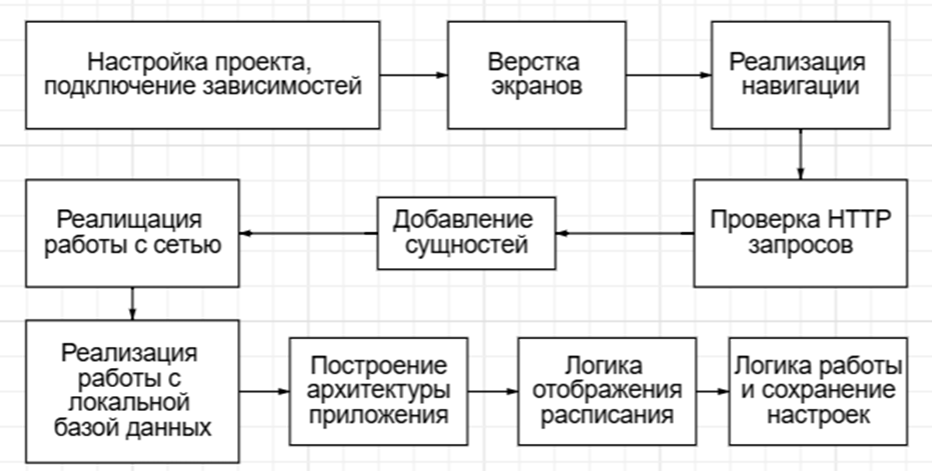
\includegraphics[width=1.0\textwidth]{1.png}
	\caption{Схема этапов реализации приложения}
	\label{fig:fig1}
\end{figure}

\subsection*{4.1. Подключение зависимостей}
\addcontentsline{toc}{subsection}{4.1. Подключение зависимостей} % Добавляем в оглавление

Для написания приложения нужно добавить необходимые библиотеки в Gradle файле на уровне приложения: 
\begin{enumerate}
	\item Retrofit – это библиотека для работы с HTTP-запросами в Android-приложениях. Она используется для взаимодействия с собственным API, обеспечивая удобный и эффективный способ отправки запросов и обработки ответов. Конвертер Gson позволяет автоматически преобразовывать JSON-ответы от API в объекты Kotlin, что упрощает работу с данными.   \cite{ref7}\cite{ref8}
	
	\item Glide – это библиотека для загрузки и отображения изображений. Она используется для отображения картинок котиков на интерфейсе, а также их кэширования для повышения производительности. \cite{ref7}
	
	\item AndroidX Libraries предоставляет современные компоненты и инструменты для разработки Android-приложений, улучшая совместимость и функциональность. \cite{ref7}
	
	\item Jetpack Compose для декларативной верстки экранов приложения. \cite{ref7}
	
	\item Jetpack Navigation: обеспечивает удобный способ навигации между экранами приложения, упрощая управление компонентами и навигационными действиями. 
	
	\item Koin – это библиотека для внедрения зависимостей, которая упрощает создание и управление зависимостями в приложении, улучшая модульность и тестируемость кода.
	
	\item Room – это библиотека для работы с базой данных SQLite, предоставляющая удобный и безопасный способ хранения и управления данными в приложении. Благодаря ей будет происходить хранение информации о треках, плейлистах и избранном.
\end{enumerate}

\subsection*{4.2. Верстка экранов}
\addcontentsline{toc}{subsection}{4.2. Верстка экранов} % Добавляем в оглавление

Все экраны приложения верстаются с помощью Kotlin Declarative подхода Jetpack Compose. На этом этапе вынесены отдельно строковые и цветовые ресурсы, необходимые шрифты и векторные изображения для иконок. Для всех частей интерфейса используются стандартные UI-элементы Android SDK.[2]
Приложение состоит из двух основных экранов: расписание и настройки. Смена состояния основного Activity с Bottom Bar осуществляется при помощи помещения одного из двух фрагментов в Scaffold. Расписание занятий отображается с помощью Column, где каждый элемент списка – это контейнер для события, куда записывается информация о занятии. Пока не начата работа с сетью, оставлены изображения-заглушки и тестовый текст, чтобы убедиться в корректности отображения интерфейса. \cite{ref8}
Для похожих элементов UI необходимо вынести одинаковые атрибуты в отдельный стиль для дальнейшего повторного использования. Также необходимо добавить поддержку светлой и темной темы, чтобы пользователи могли выбирать наиболее удобный для себя вариант отображения интерфейса. Ниже на рис. ~\ref{fig:main_screen} и рис. ~\ref{fig:settings_screen} изображена итоговая верстка экранов с тестовыми данными. \cite{ref2}


\subsection*{4.3. Реализация навигации}
\addcontentsline{toc}{subsection}{4.3. Реализация навигации} % Добавляем в оглавление
На данном этапе необходимо связать сверстанные экраны в единое приложение. Для реализации логики Bottom Bar будет использоваться Jetpack Navigation. При нажатии на элементы расписания необходимо обеспечить переход на соответствующие детальные экраны или выполнить другие действия, такие как открытие дополнительной информации о занятии. \cite{ref8}

\begin{figure}[H]
    \centering
    \begin{minipage}{0.48\textwidth}
        \centering
        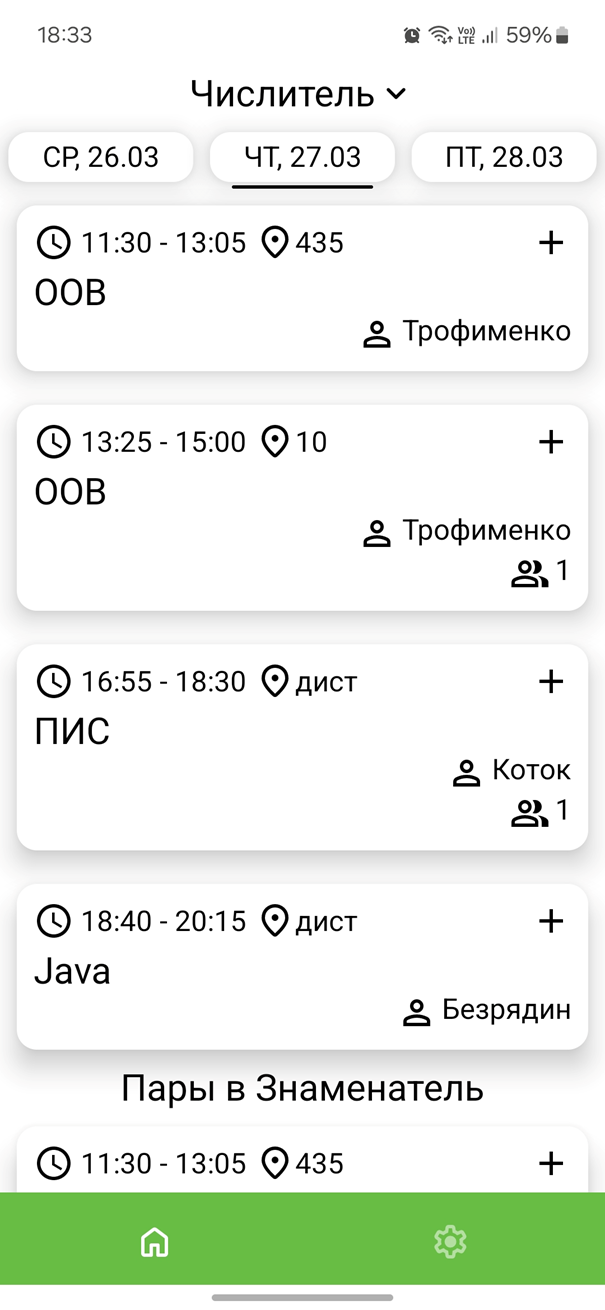
\includegraphics[width=\linewidth]{13.png}
        \caption{Макет главного экрана}
        \label{fig:main_screen}
    \end{minipage}
    \hfill
    \begin{minipage}{0.48\textwidth}
        \centering
        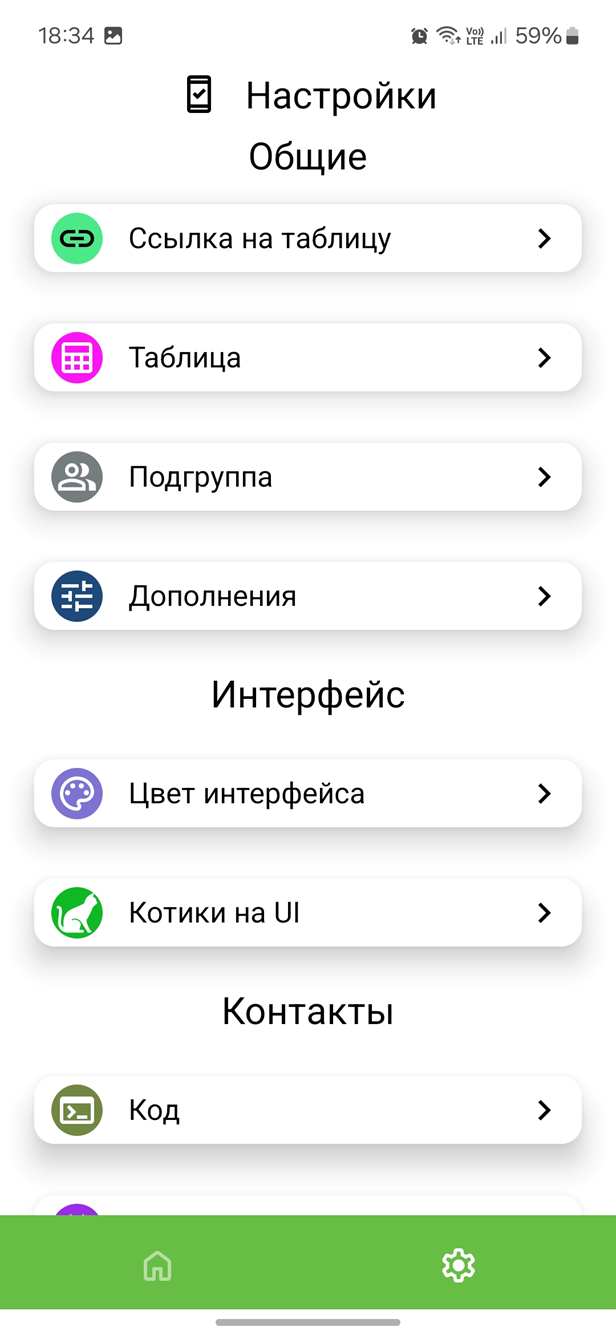
\includegraphics[width=\linewidth]{14.png}
        \caption{Макет экрана настроек}
        \label{fig:settings_screen}
    \end{minipage}
\end{figure}

На экране настроек при нажатии кнопки «Назад» необходимо вернуться на предыдущий экран. Это реализовано с помощью стандартных механизмов навигации в Android, например, NavController. \cite{ref8}
До реализации взаимодействия с базой данных полная функциональность некоторых экранов будет ограничена. Однако, основная логика навигации и переходов между экранами будет реализована для обеспечения плавного пользовательского опыта.

\subsection*{4.4. Проверка HTTP-запросов}
\addcontentsline{toc}{subsection}{4.4. Проверка HTTP-запросов} % Добавляем в оглавление

Ниже, на рис. ~\ref{fig:fig2}, рис. ~\ref{fig:fig3}, рис. ~\ref{fig:fig4}, рис. ~\ref{fig:fig5}, изображены тестовые обращения для проверки запросов к собственному API через Postman. Все данные, необходимые для отображения пользователю, существуют и корректны.  \cite{ref9}

\begin{figure}[H]
	\centering
	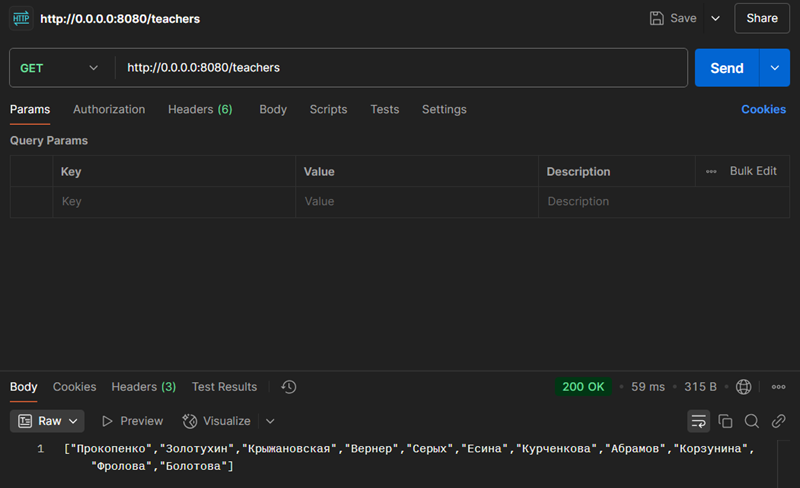
\includegraphics[width=0.8\textwidth]{2.png}
	\caption{Запрос получения преподавателей}
	\label{fig:fig2}
\end{figure}

\begin{figure}[H]
	\centering
	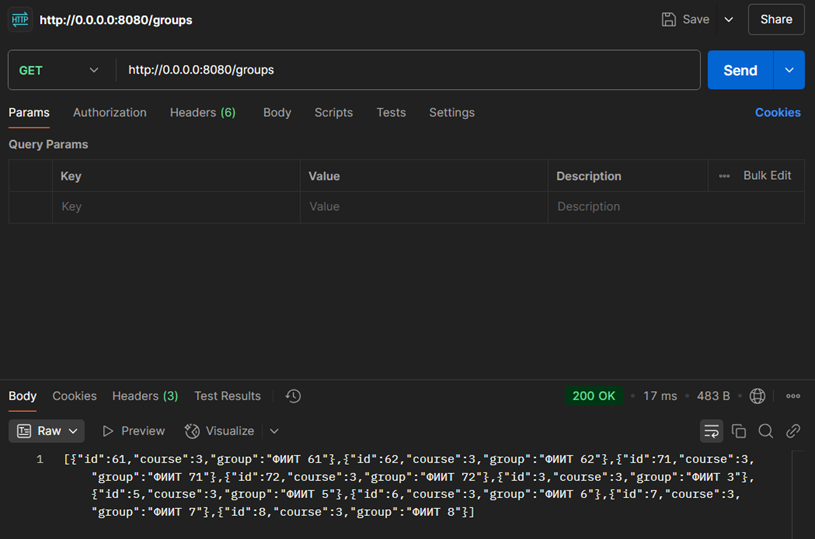
\includegraphics[width=0.8\textwidth]{3.png}
	\caption{Запрос получения групп}
	\label{fig:fig3}
\end{figure}

\begin{figure}[H]
	\centering
	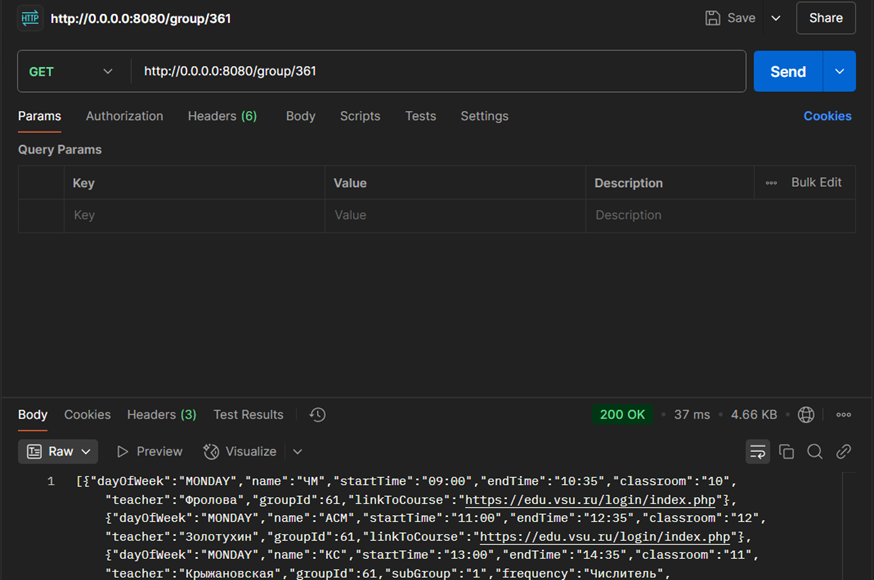
\includegraphics[width=0.8\textwidth]{4.png}
	\caption{Запрос получения расписания конкретной группы}
	\label{fig:fig4}
\end{figure}

\begin{figure}[H]
	\centering
	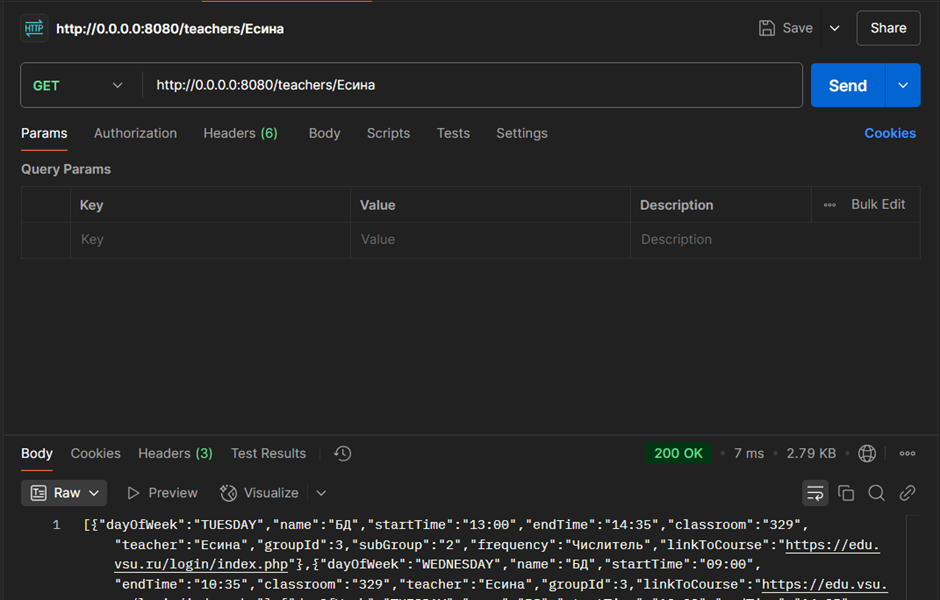
\includegraphics[width=0.8\textwidth]{5.png}
	\caption{Запрос получения расписания конкретного преподавателя}
	\label{fig:fig5}
\end{figure} 

\subsection*{4.5. Модели данных}
\addcontentsline{toc}{subsection}{4.5. Модели данных} % Добавляем в оглавление

Следующие модели данных, изображенные на рис. ~\ref{fig:fig6}, используются для конвертации в них HTTP-ответов от сервера в формате JSON и обработки для дальнейшего помещения в базу данных и отображения на интерфейсе. 
\begin{figure}[H]
	\centering
	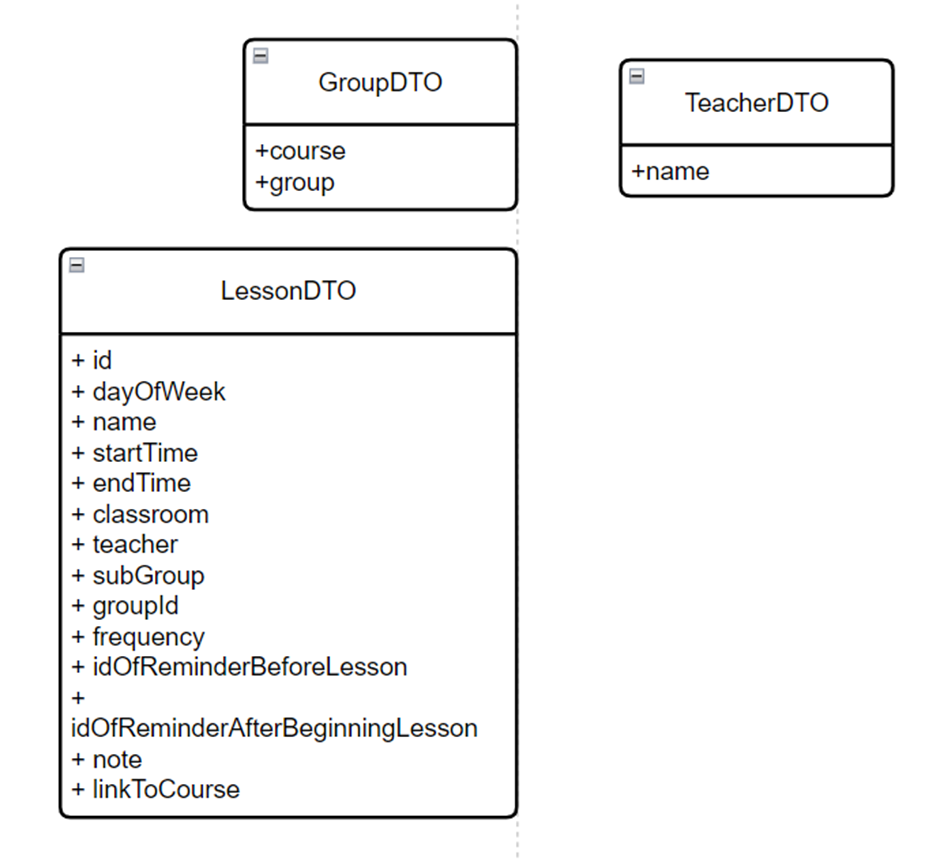
\includegraphics[width=0.7\textwidth]{6.png}
	\caption{Диаграмма классов для моделей данных сетевых репозиториев}
	\label{fig:fig6}
\end{figure} 
\begin{enumerate}
	\item LessonDto: модель для представления информации о занятии.
 	\item TeacherDto: модель для представления информации о преподавателе.
	\item GroupDto: модель для представления информации о группе студентов.
\end{enumerate}

\subsection*{4.6. Логика работы с сетью}
\addcontentsline{toc}{subsection}{4.6. Логика работы с сетью} % Добавляем в оглавление

Основная цель работы с сетью — обеспечение взаимодействия приложения с API, для получения информации о расписании по запросу пользователя. \cite{ref6}

Для работы с сетью в приложении используются следующие ключевые компоненты, диаграмма которых изображена на рис. \ref{fig:fig7}: 



\begin{enumerate}
    \item Интерфейсы LessonRemoteRepository, GroupRemoteRepository, Teacher-RemoteRepository. Определяют методы, которые принимает объект запроса и возвращает объект ответа. Эти интерфейсы позволяет абстрагироваться от конкретных деталей реализации сетевого взаимодействия, обеспечивая гибкость и возможность замены реализации при необходимости.
	
    \item Классы LessonRemoteRepositoryImpl, GroupRemoteRepositoryImpl, TeacherRemoteRepositoryImpl. Реализуют интерфейсы Lesson-RemoteRepository, GroupRemoteRepository, TeacherRemoteRepository и используют библиотеку Retrofit для выполнения сетевых запросов. Здесь проверяется сетевое подключение – прежде чем отправить запрос, проверяется наличие активного интернет-соединения. Если соединение отсутствует, возвращается ответ с соответствующим кодом ошибки. А также обрабатывается сам запрос: методы принимают параметры запроса и выполняют сетевой запрос к API. В случае успешного выполнения запроса возвращается ответ с кодом 200 и полученными данными. В случае ошибки (например, при отсутствии соединения или неверном типе запроса) возвращаются соответствующие коды ошибок.\cite{ref9}
\end{enumerate}

\begin{figure}[H]
	\centering
	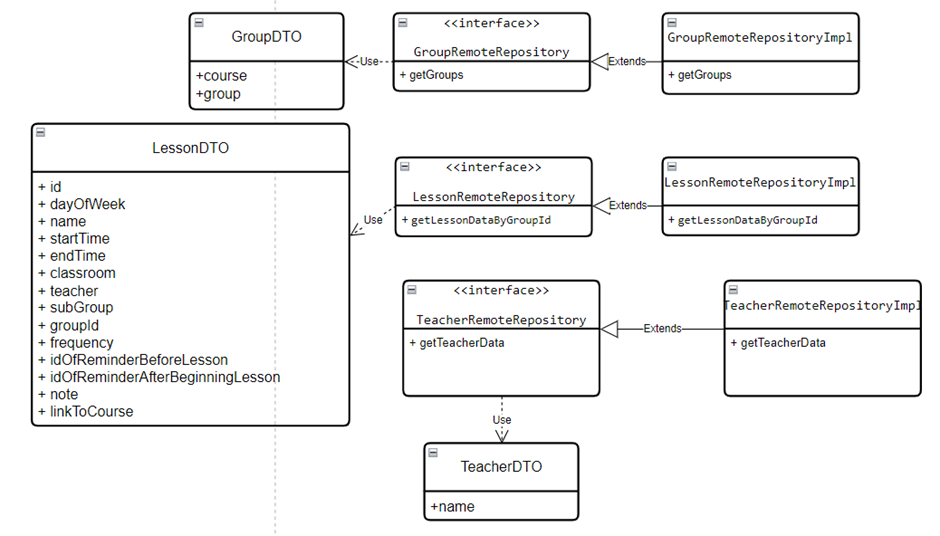
\includegraphics[width=0.8\textwidth]{7.png}
	\caption{Диаграмма классов для сетевых репозиториев}
	\label{fig:fig7}
\end{figure}

\subsection*{4.7. Логика работы с базой данных}
\addcontentsline{toc}{subsection}{4.7. Логика работы с базой данных} % Добавляем в оглавление

Для обеспечения надежного и эффективного хранения данных о занятиях в приложении используется библиотека Room, которая предоставляет удобный интерфейс для работы с SQLite базой данных в Android-приложениях. Для реализации функциональности работы с базой данных в приложении используются следующие основные компоненты:
\begin{enumerate}
	\item Entity-классы представляют собой модели данных, которые будут сохраняться в базе данных. В нашем приложении используются следующие Entity-классы, которые изображены ниже на рис. ~\ref{fig:fig8}:
		\begin{itemize}
		\item LessonEntity: представляет информацию о занятии, включая его идентификатор, название, время начала и конца, аудиторию, преподавателя и т. д.
		\item TeacherEntity: представляет информацию о преподавателе, включая его идентификатор, имя, должность и т. д.
		\item GroupEntity: представляет информацию о группе студентов, включая ее идентификатор, название и т. д.
		\item ReminderEntity: представляет информацию о напоминании о паре
		\end{itemize}
		\begin{figure}[H]
			\centering
			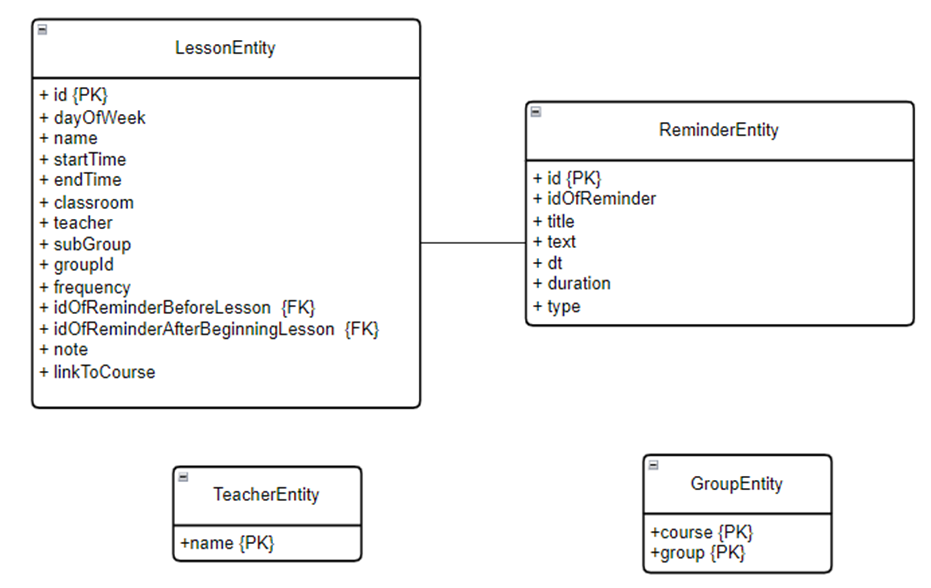
\includegraphics[width=0.8\textwidth]{8.png}
			\caption{Схема базы данных}
			\label{fig:fig8}
		\end{figure} 
		
	\item DAO (Data Access Object) интерфейсы определяют методы для взаимодействия с базой данных. В нашем приложении используются три DAO-интерфейса, которые изображены на рис ~\ref{fig:fig9}:
		\begin{itemize}
		\item LessonDao: определяет методы для вставки, удаления и получения занятий из базы данных.
		\item TeacherDao: определяет методы для вставки, удаления и получения преподавателей из базы данных.
		\item GroupDao: определяет методы для вставки, удаления и получения групп из базы данных.
		\end{itemize}
\end{enumerate}



Эти интерфейсы аннотированы с использованием аннотаций Room, таких как \texttt{@Insert}, \texttt{@Delete} и \texttt{@Query}, которые определяют SQL-запросы, выполняемые для соответствующих операций\cite{ref10}.

\begin{figure}[H]
	\centering
	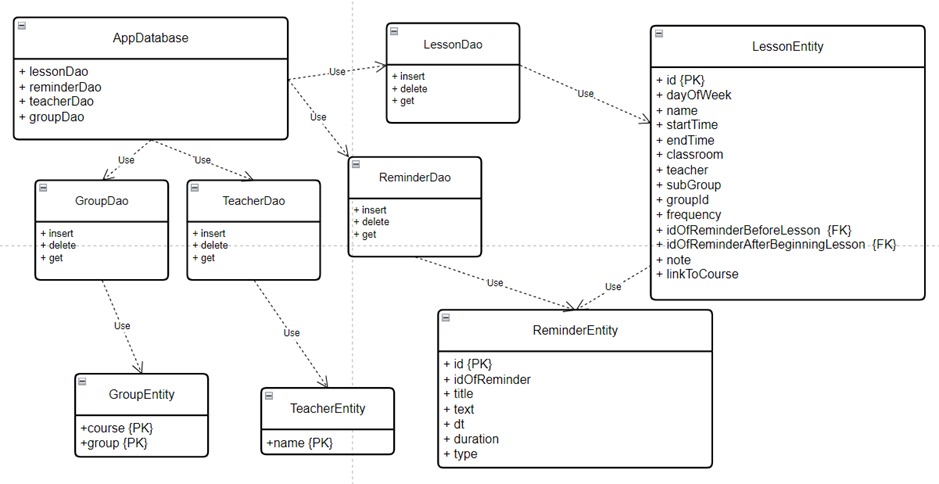
\includegraphics[width=0.8\textwidth]{9.png}
	\caption{Диаграмма классов базы данных}
	\label{fig:fig9}
\end{figure} 


\begin{enumerate}[start=3]
    \item Абстрактный класс базы данных наследуется от \texttt{RoomDatabase} и представляет собой точку входа для взаимодействия с базой данных. В нашем приложении определены следующие классы:
    
    \begin{itemize}
        \item AppDatabase: абстрактный класс для работы с таблицей занятий. Содержит абстрактные свойства \texttt{lessonDao}, \texttt{groupDao}, \texttt{teacherDao}, возвращающие экземпляры интерфейсов \texttt{LessonDao}, \texttt{GroupDao} и \texttt{TeacherDao} соответственно.
    \end{itemize}

    \item Клиент базы данных предоставляет методы для взаимодействия с базой данных через DAO-интерфейсы. В нашем приложении используется класс \texttt{AppDatabase\_Impl}, который реализует интерфейс \texttt{AppDatabase}. Этот класс определяет методы для сохранения, удаления и получения занятий. Класс \texttt{AppDatabase\_Impl} инкапсулирует логику работы с базой данных, обеспечивая удобный интерфейс для других компонентов приложения. Он использует инъекцию зависимости для получения экземпляра базы данных и обеспечивает выполнение CRUD-операций через соответствующие DAO-интерфейсы.
\end{enumerate}


\subsection*{4.8. Архитектура приложения}
\addcontentsline{toc}{subsection}{4.8. Архитектура приложения} % Добавляем в оглавление

Приложение будет разработано с соблюдением принципов SOLID и чистой архитектуры. Применение этих принципов обеспечивает высокую степень модульности, гибкости и тестируемости кода, а также упрощает поддержку и расширение функциональности~\cite{ref3}.

Чистая архитектура разделяет систему на несколько слоев, каждый из которых имеет чётко определённые задачи и зависимости. Это позволяет легко изменять и масштабировать приложение, а также улучшает его тестируемость. В соответствии с чистой архитектурой в приложении выделены следующие основные слои:

\begin{enumerate}
    \item \textbf{Внешний слой (UI Layer)}: включает все компоненты, связанные с пользовательским интерфейсом, такие как фрагменты и активности. Основная задача UI Layer - отображение данных и взаимодействие с пользователем. Этот слой получает данные из ViewModel и обновляет интерфейс в соответствии с изменениями в данных~\cite{ref3}.
    \item \textbf{Слой данных (Data Layer)}: содержит компоненты, связанные с управлением данными, включая DAO-интерфейсы для работы с Room, реализации сетевых запросов с использованием Retrofit, а также клиентов базы данных и сетевых клиентов. Data Layer отвечает за получение и хранение данных, предоставляя их в Domain Layer через репозитории~\cite{ref3}.
    \item \textbf{Слой домена (Domain Layer)}: содержит бизнес-логику и бизнес-модели. Domain Layer не зависит от других слоев и содержит основные бизнес-правила и интерфейсы репозиториев~\cite{ref3}.
    \item \textbf{Слой приложений (Application Layer)}: содержит ViewModel, которые объединяют бизнес-логику с логикой представления и управления состоянием. ViewModel взаимодействуют с репозиториями для получения данных и обработки пользовательских действий.
\end{enumerate}

Для разделения представления и логики управления данными в приложении используется паттерн MVVM (Model-View-ViewModel). Этот паттерн обеспечивает чёткое разделение обязанностей между компонентами приложения:

\begin{enumerate}
    \item \textbf{Model}: включает бизнес-логику и данные приложения. Модель получает данные из Data Layer и предоставляет их ViewModel.
    \item \textbf{View}: состоит из пользовательского интерфейса и отвечает за отображение данных. View наблюдает за изменениями в ViewModel и обновляет интерфейс в соответствии с этими изменениями.
    \item \textbf{ViewModel}: посредник между View и Model. ViewModel запрашивает данные у Model и предоставляет их View, а также обрабатывает пользовательские действия и обновляет Model.
\end{enumerate}

Для управления зависимостями и их внедрения в приложении используется библиотека Koin. В модулях Koin определяются зависимости и способы их создания. Например, можно определить зависимости для сетевого клиента, базы данных и ViewModel. Это позволяет централизованно управлять зависимостями и облегчает их модификацию. Koin автоматически предоставляет экземпляры классов, когда они требуются, что упрощает тестирование и модульность. Например, ViewModel могут получать необходимые репозитории через Koin, что устраняет жёсткие зависимости\cite{ref10}

\newpage
\section*{5. Основная логика работы приложения}
\addcontentsline{toc}{section}{5. Основная логика работы приложения} % Добавляем в оглавление
Основную логику работы приложения, которая изображена ниже на рис. ~\ref{fig:fig10}, можно разделить на 2 части:
\begin{enumerate}
	\item Просмотр информации о занятиях
	\item Изменение настроек приложения
\end{enumerate}

\begin{figure}[H]
	\centering
	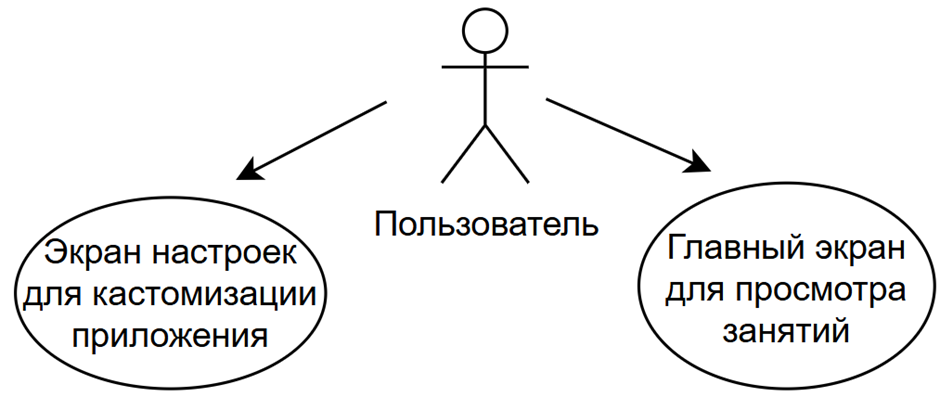
\includegraphics[width=0.8\textwidth]{10.png}
	\caption{Диаграмма вариантов использования приложения}
	\label{fig:fig10}
\end{figure} 

\subsection*{5.1. Логика работы компонента «Главный экран»}
\addcontentsline{toc}{subsection}{5.1. Логика работы компонента «Главный экран»} % Добавляем в оглавление

Логика работы просмотра расписания в приложении реализована через несколько ключевых компонентов: интерфейсы, реализации и клиенты. Функциональность главного экрана можно увидеть на соответствующей иллюстрации (рис.~\ref{fig:fig11}).
Эти компоненты взаимодействуют друг с другом для обеспечения функциональности отображения актуального расписания на сегодня, на другие дни, редактирования заметок. При разработке логики получения расписания важно учитывать несколько ключевых моментов, таких как получение данных от удаленного сервера, обработка ответа, управление локальными данными и обеспечение удобного пользовательского интерфейса. В нашем приложении мы используем MVVM архитектуру и DI с помощью Koin для организации кода.

Весь процесс можно разбить на следующие основные компоненты \cite{ref10}: 
\begin{enumerate}
    \item Репозитории данных об учебных занятиях, преподавателях и группах (\texttt{LessonRemoteRepository}, \texttt{GroupRemoteRepository}, \\  \texttt{TeacherRemoteRepository}): эти компоненты отвечают за взаимодействие с данными от удаленного сервера об учебных занятиях, преподавателях и группах. Они осуществляют запросы к удаленному серверу. 
    \item Локальные репозитории данных об учебных занятиях, преподавателях и группах (\texttt{LessonLocalRepository}, \texttt{GroupLocalRepository}, \\  \texttt{TeacherLocalRepository}): эти компоненты отвечают за взаимодействие с локальной базой данных и реализуют операции чтения/записи данных, которые приходят с сервера для кэширования и работы приложения без интернета.
\end{enumerate}

\begin{figure}[H]
    \centering
    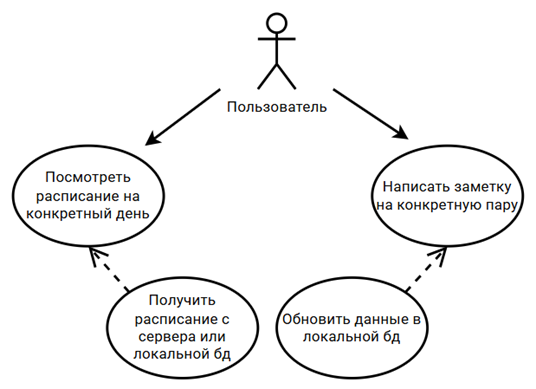
\includegraphics[width=0.8\textwidth]{11.png}
    \caption{Диаграмма вариантов использования компонента «Главный экран»}
    \label{fig:fig11}
\end{figure}

\subsection*{5.2. Логика работы компонента «Настройки»}
\addcontentsline{toc}{subsection}{5.2 Логика работы компонента «Настройки»} % Добавляем в оглавление


Компонент настроек (SettingsScreen) отвечает за предоставление пользователю возможности изменять параметры приложения, такие как тема оформления, а также за доступ к некоторым внешним ресурсам, например поддержке.

Весь процесс можно разбить на следующие основные компоненты:
\begin{enumerate}
    \item Компонент «Настройки» (\texttt{SettingsScreen}): фрагмент, отвечающий за отображение и управление настройками приложения. Он содержит интерфейс для изменения темы, отправки отзывов, просмотра пользовательского соглашения и т. д.
    \item \texttt{SettingsScreenViewModel}: ViewModel, который обрабатывает бизнес-логику, связанную с настройками. Он взаимодействует с репозиторием и юзкейсами для получения и сохранения данных.
    \item Менеджер настроек (\texttt{SettingsManager}): интерфейс, определяющий методы для доступа к хранилищу данных настроек. Включает методы для сохранения и получения данных настроек, а также для изменения темы.
    \item Хранилище настроек (\texttt{SharedPreferences}): реализация хранилища настроек, которую использует \texttt{SettingsManager} для сохранения настроек.
\end{enumerate}

\begin{figure}[H]
    \centering
    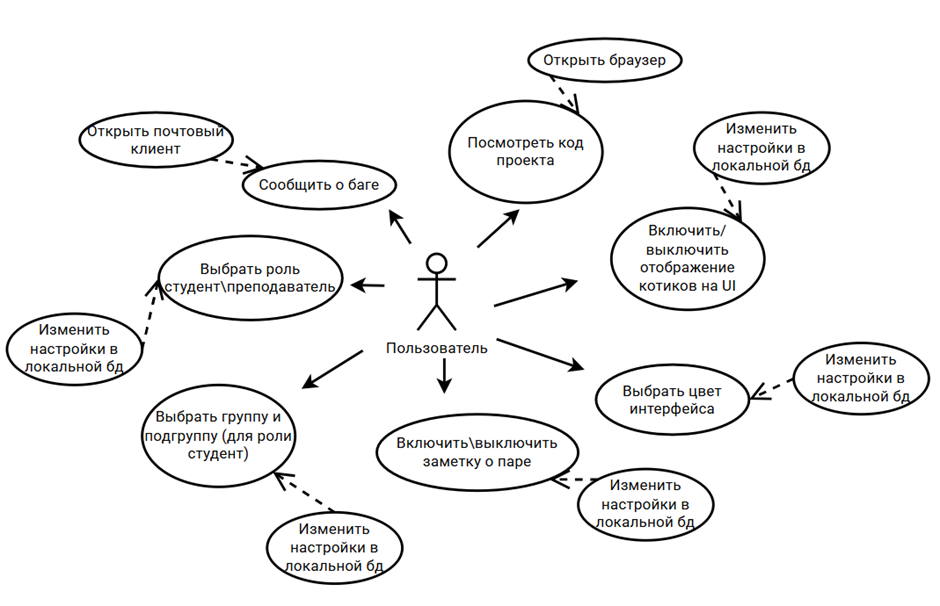
\includegraphics[width=0.8\textwidth]{12.png}
    \caption{Диаграмма вариантов использования компонента «Настройки»}
    \label{fig:fig12}
\end{figure}

Взаимодействие с компонентом настроек, изображенное на рис. \ref{fig:fig12}, производится в соответствии со следующим планом:
\begin{itemize}
    \item При открытии компонента на экране создается пользовательский интерфейс, и он связывается с ViewModel. Это обеспечивает связь между отображаемыми данными и бизнес-логикой. При загрузке компонента текущие настройки (например, состояние переключателя темы) запрашиваются из ViewModel. ViewModel получает данные \\ от \texttt{SettingsManager}, который взаимодействует с хранилищем. Текущие настройки отображаются в интерфейсе.
    \item Пользователь взаимодействует с элементами интерфейса, такими как переключатель темы, кнопки для отправки отзывов или просмотра кода приложения, а также выбор роли/группы/подгруппы. Когда пользователь изменяет состояние переключателя темы, новое состояние сохраняется через ViewModel и \texttt{SettingsManager}. Тема приложения немедленно обновляется, чтобы отразить новое состояние. При нажатии на соответствующие элементы интерфейса ViewModel вызывает методы интерактора для выполнения этих действий. Юзкейс использует внешний навигатор для отправки письма, открытия ссылки или браузера. После изменения настроек интерфейс обновляется, чтобы отразить текущие параметры. Например, после переключения темы приложение немедленно переключается в дневной или ночной режим.
    \item Все изменения настроек сохраняются в хранилище данных через репозиторий. Это гарантирует, что при следующем запуске приложения будут применены последние сохранённые настройки.
\end{itemize}

\newpage
\begin{center}
	\textbf{Заключение}
\end{center}
\addcontentsline{toc}{section}{Заключение} % Добавляем в оглавление

Было разработано мобильное приложение, которое позволяет просматривать расписание университета. Также была реализована возможность добавлять заметки к учебным занятиям, изменять цвет интерфейса, сообщать об ошибках и просматривать код приложения.

Данное решение может быть масштабировано путём добавления расширенного функционала. В первую очередь это настройка персонализированного отображения пар, например, не списком, а в виде таблицы. Также может быть добавлена система аккаунтов для сохранения настроек на сервере, что позволит синхронизировать их между устройствами одного пользователя.

% Окружение библиографии
\renewcommand{\refname}{Список используемых источников}
\bibliography{sources}

\newpage
\begin{center}
	\textbf{Приложения}
\end{center}
\addcontentsline{toc}{section}{Приложения} % Добавляем в оглавление


\lstinputlisting[
    language=Kotlin,
    caption={Главный класс приложения},
    label={lst:codekt},
    firstline=1,
    lastline=17
]{code.kt}


\lstinputlisting[
    language=Kotlin,
    caption={Компонент с логикой для главного класса приложения},
    label={lst:codekt},
    firstline=18,
    lastline=116
]{code.kt}

\lstinputlisting[
    language=Kotlin,
    caption={Главный экран},
    label={lst:codekt},
    firstline=117,
    lastline=446
]{code.kt}

\lstinputlisting[
    language=Kotlin,
    caption={Экран настроек},
    label={lst:codekt},
    firstline=448,
    lastline=861
]{code.kt}

\end{document}
